\documentclass[letterpaper,twocolumn,openany,nodeprecatedcode]{dndbook}
\usepackage[english]{babel}
\usepackage[utf8]{inputenc}
\usepackage{pdfpages}
\usepackage{graphicx}
\usepackage{wrapfig}
\usepackage{color}
\usepackage{tikz}
\usepackage{lipsum}
\usepackage{hyperref}
\usepackage{titling}
\usepackage{pagecolor}
\usepackage{afterpage}
\usepackage{titletoc}
\usepackage{everyshi}

\title{
    Homebrew Brews\\
    \large A compendium of Magical Mixtures and Fantastical Elixirs\\
    Part X\\%
    \begin{tikzpicture}[remember picture]\\%
        \node (main) {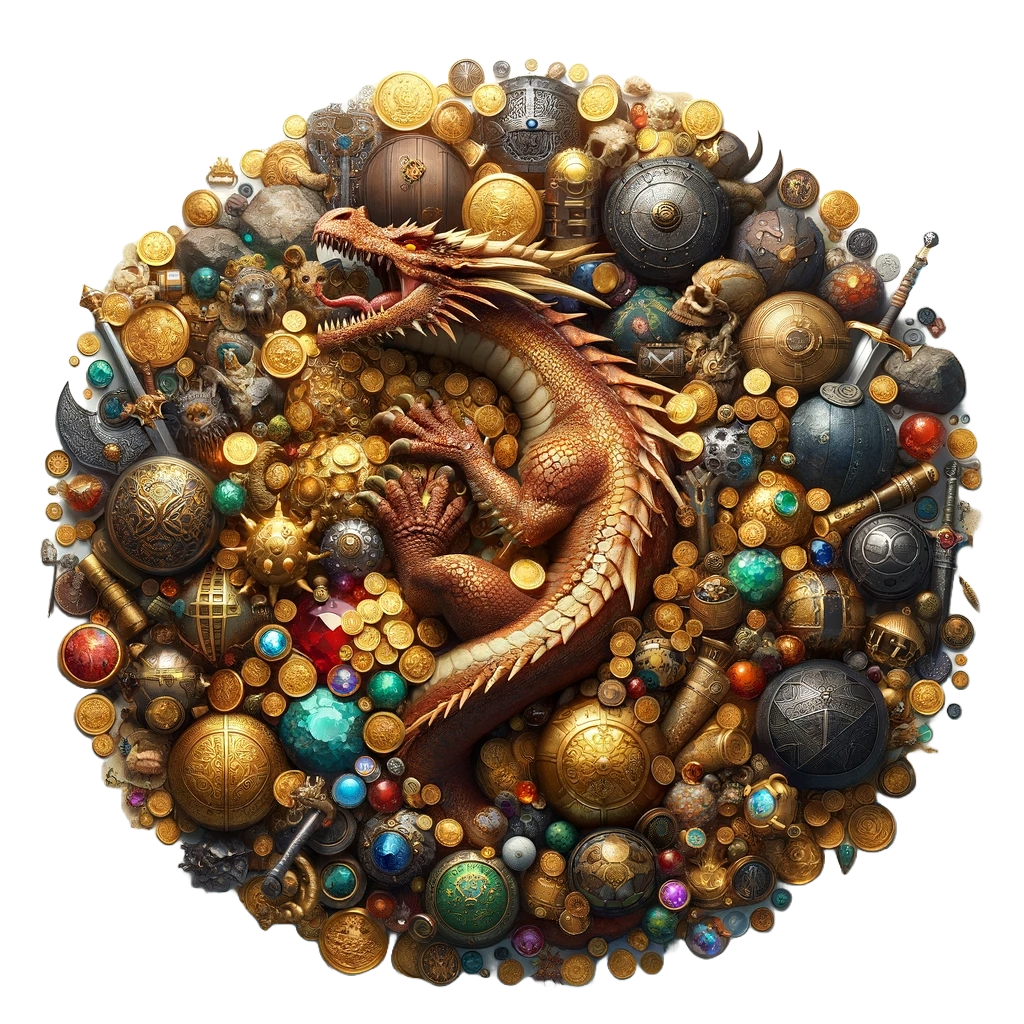
\includegraphics[width=4in]{img/inside_cover.png}};\\%
    \end{tikzpicture}
    }

\author{\large Jackson Dean and Rae Gehman}
\date{}


\begin{document}


% \frontmatter
\maketitle


\onecolumn
\section{Credits}
\begin{itemize}
    \item[] 
\textbf{Authors:} Jackson Dean and Rae Gehman
% \item[]
% \textbf{Artists:} TBD
% \item[]
% \textbf{Maps:} 
\end{itemize}

\vspace*{\fill}
\begin{figure}[h]
\centering
    
\includegraphics[width=2in]{img/available_dms_guild.png}
\end{figure}
\vspace*{\fill}

\newcommand\blfootnote[1]{%
  \begingroup
  \renewcommand\thefootnote{}\footnote{#1}%
  \addtocounter{footnote}{-1}%
  \endgroup
}
\blfootnote{ 
    DUNGEONS \& DRAGONS, D\&D, Wizards of the Coast, Forgotten Realms, Ravenloft, Eberron, the dragon ampersand, Ravnica and all other Wizards of the Coast product names, and their respective logos are trademarks of Wizards of the Coast in the USA and other countries.    
    This work contains material that is copyright Wizards of the Coast and/or other authors. Such material is used with permission under the Community Content Agreement for Dungeon Masters Guild.
    All other original material in this work is copyright 2023 by Jackson Dean and published under the Community Content Agreement for Dungeon Masters Guild.
}

\twocolumn

\tableofcontents


\chapter*{Introduction}
\addcontentsline{toc}{chapter}{Introduction}
\markboth{Introduction}{}

\section{The Joy of Potion Brewing}
    Potion brewing is not just for stuffy old wizards! It's a delightful hobby that can lead to explosive results (sometimes literally). In this book, you'll discover how to mix, stir, and brew your way to magical mastery. Remember, every great potion starts with a bit of fun and a sprinkle of adventure.

\section{Potion Crafting Mechanics}
Crafting a potion is as easy as pie - magical pie! Here's what you need to know:
\begin{itemize}
  \item \textbf{Ingredients' Gold Cost:} Every potion starts with ingredients. You'll need to invest some gold to gather what you need. The rarer the potion, the pricier the components!
  \item \textbf{Brewing Time:} Patience is key! Brewing takes time, ranging from an hour for a simple potion to several days for something truly spectacular.
  \item \textbf{Alchemy Tools Check:} Roll those dice! The success of your potion depends on an Alchemy Tools check. The DC varies based on the potion's complexity. Fail a check and you lose the time required to craft the potion, fail by five or more and you also lose the ingredients. Alternatively, a failed roll might result in additional effects under \textit{botched crafting effects}.
  \item \textbf{Crafting During Downtime:} Brew your potions during downtime or while resting. 
\end{itemize}

The DC for any saving throws is 8 + your proficiency bonus + your Intelligence or Wisdom (your choice).

\section{Understanding Potion Recipes}
    Each potion recipe in this book comes with a suggested cost of ingredients, the time needed to brew it, and the Alchemy Tools DC. 

\section{A Pinch of Caution}
    While potion brewing is a barrel of laughs, it's not without risks. A botched potion can have unintended effects, so always wear your safety goggles and keep a cat or toad nearby for good luck!

\section{Embarking on the Brewing Adventure}
    Ready to become a master potion brewer? Let's turn the page and start our whimsical adventure in the magical world of potions!

\begin{tikzpicture}[remember picture,overlay]\\%
    \node (main) [xshift=2.5in,yshift=-5in] {
\includegraphics[height=.8\paperheight]{img/intro.png}};\\%
\end{tikzpicture}




\chapter{Potions}

\DndItemHeader{<POTION NAME>}{xxx potion}
<DESCRIPTION OF APPEARENCE AND EFFECT>

\textbf{Crafting:} XX gp | X hours | DC X \\
\textbf{Botched Brewing Effect:} XXX



Great now put these into this format for a d100 table. There will eventually be 50 items in the table, so each entry should have 2 numbers:



\begin{DndTable}[header=<HEADER>]{cX}
  \textbf{d100} & \textbf{<HEADER>} \\
  1-2 & \textbf{<NAME*>}: <DESCRIPTION>\\
    3-4 & ...

put an asterisk next to items that require attument and make sure to include two backslashes per row "\\"

Do not write "requires" attunement at the end


*************************************
You are an expert-level creative game designed for D&D 5e.
Let's make some magic <ITEM> for D&D 5th edition. I want all of them to be completely unique, never-before seen creative, fun, well-balanced items.

Send me ideas for <ITEM>. For each one, include specific mechanics, flavor description, and lore.

Then for each one, give a separate breakdown for how it is a unique, never-before seen <ITEM> that creatively blends mechanics and lore to make add an interesting twist to a D&D campaign. Never repeat the same idea more than once. Let's bring some items to life! 

Start by sending 5 <ITEM> and their breakdowns
    step 1) Uniqueness
    step 2) Comparison to other items
    step 3) Name, brief detailed description of appearance, concrete/detailed mechanics and one sentence of interesting lore. Use complete sentences.

If you create any new effects, briefly describe what they do in parenthesis, including what kind of save or spell attack and any effects/damage and the DC. Also specify what type of action (if any) activating an item takes.

Each one should be more complex then just "cast this spell once per day". Instead, they should offer a unique thematic twist on mechanics that make them interesting, well-balanced and  worthwhile <ITEM>

Do not rely too heavily on existing tropes. Make each one surprising and unexpected.

AVOID THE FOLLOWING CONCEPTS LISTED BETWEEN "[" and "]":
    [whispers], [echos], [dreamweaver], [chameleon], [rift], [wind], [shadows]

Here are some examples of some items from various item categories:

```examples
 \itemrow{Celestial Glaive}\rarity{Weapon (glaive)}{rare}{true} & This +1 brilliant silver glaive emits a burst of blinding starlight on a critical hit. The target makes a DC 15 Constitution saving throw to resist blindness, and can repeat the save at end of each turn if they fail. At night, it deals an extra 1d6 radiant damage, its blade trailing celestial light with each swing. Forged from a fallen star, it carries the essence of the night sky. \\

  \itemrow{Ring of the Mountaineer}\rarity{Ring}{uncommon}{true} & This ring made from rough stone grants the ability to climb surfaces without needing to make checks. Wisdom (Perception) checks made while attuned to this ring while at an altitude of over 6,000 feet have advantage. Found at the peak of a mountain by a climber who wanted nothing more than to touch the sky.\\

  \itemrow{Figurine of the Celestial Stag}\rarity{Adventuring Gear (Wondrous Item)}{uncommon}{true} & This delicate silver statuette transforms into a large, celestial stag with stars shimmering in its fur. Once per day, it can be activated to provide guidance, acting as a \textit{find the path} spell as the stag communicates through visions. Crafted by a friendly forest deity, this stag once guided lost souls through spiritual journeys in the woods. While attuned to this item, a creature can cast the \textit{guidance} spell, targeting only creatures which have not done significant harm to nature. \\

  
      \itemrow{The Golden Goblet of Greed}\rarity{Adventuring Gear (Wondrous Item)}{very rare}{false} & An ostentatious golden goblet that induces craving for any non-poisonous liquid that it contains. A creature that drinks from the goblet makes a DC 17 Wisdom saving throw. On a failure, the creature is incapacitated as they use their turns drinking from the goblet as quickly as possible. They can repeat the save at the end of their turns, ending the effect on a success. If they drink from the goblet for more than one turn in a row, they begin to suffocate and will fall unconscious after a number of rounds equal to their constitution modifier (minimum of two) unless they succeed on the Wisdom save.   \\


```
**************

Format the items into latex, continuing the number sequence. Include the entire mechanics, flavor, and lore text in the latex, word for word in complete sentences. This is the format for a d100 table.
    ```latex
    \begin{DndTable}[header=<HEADER>]{c s B}
      itemrow{<NAME>}\rarity{<TYPE OF ITEM>}{<RARITY>}{<'true' or 'false' FOR ATTUNEMENT>} & <DESCRIPTION> \\

      ...
    ```

here is an example:
```example

      \itemrow{The Golden Goblet of Greed}\rarity{Adventuring Gear (Wondrous Item)}{very rare}{false} & An ostentatious golden goblet that induces craving for any non-poisonous liquid that it contains. A creature that drinks from the goblet makes a DC 17 Wisdom saving throw. On a failure, the creature is incapacitated as they use their turns drinking from the goblet as quickly as possible. They can repeat the save at the end of their turns, ending the effect on a success. If they drink from the goblet for more than one turn in a row, they begin to suffocate and will fall unconscious after a number of rounds equal to their constitution modifier (minimum of two) unless they succeed on the Wisdom save.   \\

```
    
    subsequent entries past the first 5 do not need the \begin{DndTable} header
    make sure to include two backslashes per row "\\"
use \textit for any official spell names

    Do not write "requires attunement" at the end

    make sure to put the FULL EXACT text from step 1 in the latex, DO NOT paraphrase or summarize! USE COMPLETE SENTENCES.

    <RARITY> should be one of common, uncommon, rare, very rare, legendary based on what tier of play the item is designed for.

    Legendary is reserved for only the most extraordinary items.

*********************

... or make them use the theme of ""

...

\begin{tikzpicture}[remember picture,overlay]\\%
    \node [anchor=south east] at (current page.south east) [xshift=0.20in, yshift=-0.20in] {\includegraphics[height=.55\textwidth]{img/adventures.png}};\\%
\end{tikzpicture}



\end{document}